\documentclass[12pt, a4paper]{article}
\usepackage[T2A]{fontenc}
\usepackage[utf8]{inputenc}
\usepackage[russian]{babel}
\usepackage{amsmath, amssymb} % AMS packages for math
\usepackage{graphicx}        % Required for including images
\usepackage{geometry}        % For setting margins
\geometry{left=2cm, right=1.5cm, top=2cm, bottom=2cm}
\usepackage{float}           % For better figure placement ([H] option)
\usepackage[labelsep=colon]{caption} % For figure/table captions
\usepackage{siunitx}         % For units (use \SI{value}{unit})
% Setup siunitx for Russian comma decimal separator
\sisetup{output-decimal-marker={,}}

% For plotting directly in LaTeX (optional, requires pgfplots package)
\usepackage{pgfplots}
\pgfplotsset{compat=1.18} % Use a recent compatibility mode

\begin{document}

% --- Custom Title Block ---
\begin{center}
\textsc{Санкт-Петербургский национальный исследовательский институт информационных технологий, механики и оптики\\[3mm]
Физический факультет} \\[3mm]
\end{center}
\vspace{5mm}
\line(1,0){\textwidth}
\begin{center}
\textbf{ЛАБОРАТОРНАЯ РАБОТА №2.10\\}
\textbf{"Измерение теплоты парообразования воды"}
\end{center}
\vspace{2mm}
\line(1,0){\textwidth}
\vspace{5mm}
% --- Student Info ---
\begin{minipage}{0.4\textwidth}
    Группа: Z3144 \\
    Студент: Турчанин Евгений\\
    \vspace{1mm}
\end{minipage}
\vspace{1cm}

% --- Section 1: Goals ---
\section{Цели работы}
\begin{enumerate}
    \item Измерение теплоты парообразования воды.
\end{enumerate}
\vspace{0.5cm}

% --- Section 2: Tasks ---
\section{Задачи, решаемые при выполнении работы}
\begin{enumerate}
    \item Прямое измерение массы испаряющейся жидкости при передаче ей тепла.
    \item Определение полезной мощности счетчика электроэнергии.
    \item Построение графика зависимости работы измерительного модуля от массы испарившейся воды.
    \item Определение удельной теплоты парообразования воды.
\end{enumerate}
\vspace{0.5cm}

% --- Section 3: Formulas and Initial Data ---
\section{Рабочие формулы и исходные данные}
\subsection*{Рабочие формулы}
\begin{enumerate}
    \item Количество теплоты, необходимое для превращения жидкости в пар:
    \begin{equation} \label{eq:Q_Lm}
        Q = Lm
    \end{equation}
    где $L$ - удельная теплота парообразования (Дж/кг), $m$ - масса испарившейся воды (кг).

    \item Мощность тепловых потерь в окружающую среду (мощность охлаждения):
    \begin{equation} \label{eq:N_okr}
        N_{\text{окр}} = \frac{cM\Delta t}{\tau}
    \end{equation}
    где $c$ - удельная теплоемкость воды, $M$ - масса воды в сосуде (кг), $\Delta t$ - изменение температуры измерительного модуля за время $\tau$ при охлаждении (°C), $\tau$ - время охлаждения (с).

    \item Полная электрическая мощность, выделяемая ТЭНом:
    \begin{equation} \label{eq:N_poln}
        N_{\text{полн}} = \frac{U^2}{R}
    \end{equation}
    где $U$ - напряжение сети (В), $R$ - сопротивление ТЭНа при температуре кипения (Ом).

    \item Полезная мощность, идущая на парообразование:
    \begin{equation} \label{eq:P}
        P = N_{\text{полн}} - N_{\text{окр}}
    \end{equation}

    \item Работа, совершенная за счет полезной мощности за время $t$:
    \begin{equation} \label{eq:A_Pt}
        A = P \cdot t
    \end{equation}
    где $t$ - время кипения (с).
    Теоретически, эта работа равна количеству теплоты, пошедшему на испарение: $A \approx Q$. Следовательно, $P \cdot t \approx L \cdot m$. Отсюда удельная теплота парообразования может быть найдена как:
    \begin{equation} \label{eq:L_At_m}
        L = \frac{A}{m} = \frac{P \cdot t}{m}
    \end{equation}
    или как тангенс угла наклона графика зависимости $A(m)$:
    \begin{equation} \label{eq:L_slope}
        L = \frac{\Delta A}{\Delta m}
    \end{equation}
\end{enumerate}

\subsection*{Исходные данные}
\begin{enumerate}
    \item Измерительный модуль охлаждается на $\Delta t = \SI{10}{\degree C}$ за время $\tau = 2 \text{ минуты} = \SI{120}{с}$.
    \item Масса воды в сосуде с ТЭНом $M \approx 1 \text{ литр} \approx \SI{1}{кг}$ (примем \SI{1}{кг} для расчета $N_{\text{окр}}$).
    \item Удельная теплоемкость воды $c = \SI{4200}{Дж/(кг \cdot \degree C)}$.
    \item При температуре кипения ($\approx \SI{100}{\degree C}$): сопротивление $R = \SI{82}{Ом}$, напряжение $U = \SI{232}{В}$.
    \item Табличное значение удельной теплоты парообразования воды при \SI{100}{\degree C}: $L_{\text{табл}} = \SI{2,26e6}{Дж/кг} = \SI{2,26}{МДж/кг}$.
\end{enumerate}
\vspace{0.5cm}

% --- Section 4: Experimental Setup ---
\section{Экспериментальная установка}
Внешний вид установки представлен на Рис.
\begin{figure}[H]
    \centering
    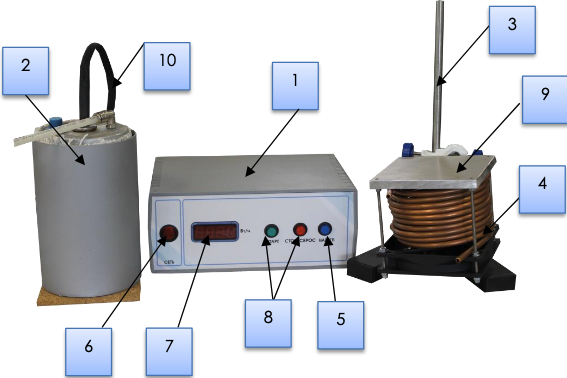
\includegraphics[width=0.8\textwidth]{fig_1} % Changed filename
    \caption{Внешний вид установки: 1 - измерительный модуль (счетчик электроэнергии); 2 - сосуд с ТЭНом; 3 - стойка с основанием; 4 - охлаждающий элемент; 5 - кнопка «нагрев»; 6 - кнопка включения стенда «Сеть»; 7 - панель индикации; 8 - кнопки управления счетчика «Старт/Стоп» и «Сброс»; 9 - конденсатор пара; 10 - мерная трубка.}
    \label{fig:setup}
\end{figure}
\vspace{0.5cm}

% --- Section 5: Measuring Instruments ---
\section{Измерительные приборы}
\begin{table}[H]
    \centering
    \caption{Основные измерительные средства}
    \label{tab:instruments}
    \begin{tabular}{|c|l|c|c|}
        \hline
        № & Наименование средства измерения & Предел измерений & Погрешность \\
        \hline
        1 & Панель индикации на счетчике электроэнергии & - & \SI{0,05}{Вт \cdot ч} \\
        2 & Мерный стакан (для оценки объема) & до \SI{100}{мл} & \SI{2,5}{мл} \\
        3 & Весы (для измерения массы испарившейся воды) & - & \SI{5}{мг} (предполагается) \\
        4 & Секундомер (встроенный или внешний) & - & \SI{0,01}{с} (предполагается) \\
        \hline
    \end{tabular}
\end{table}
\vspace{0.5cm}

% --- Section 6: Results and Processing ---
\section{Результаты измерений и их обработка}

Из стенда: $P = 200$ Вт (приборная мощность).
Тогда работа $A = Pt = 200*1072\approx 214458$
Так как почти вся работа идет на испарение, то $A \approx Lm$. Откуда $L = A/m \approx 2144580 = 2.14\cdot10^6$

\section{Графики}
\begin{figure}[H]
    \begin{center}
    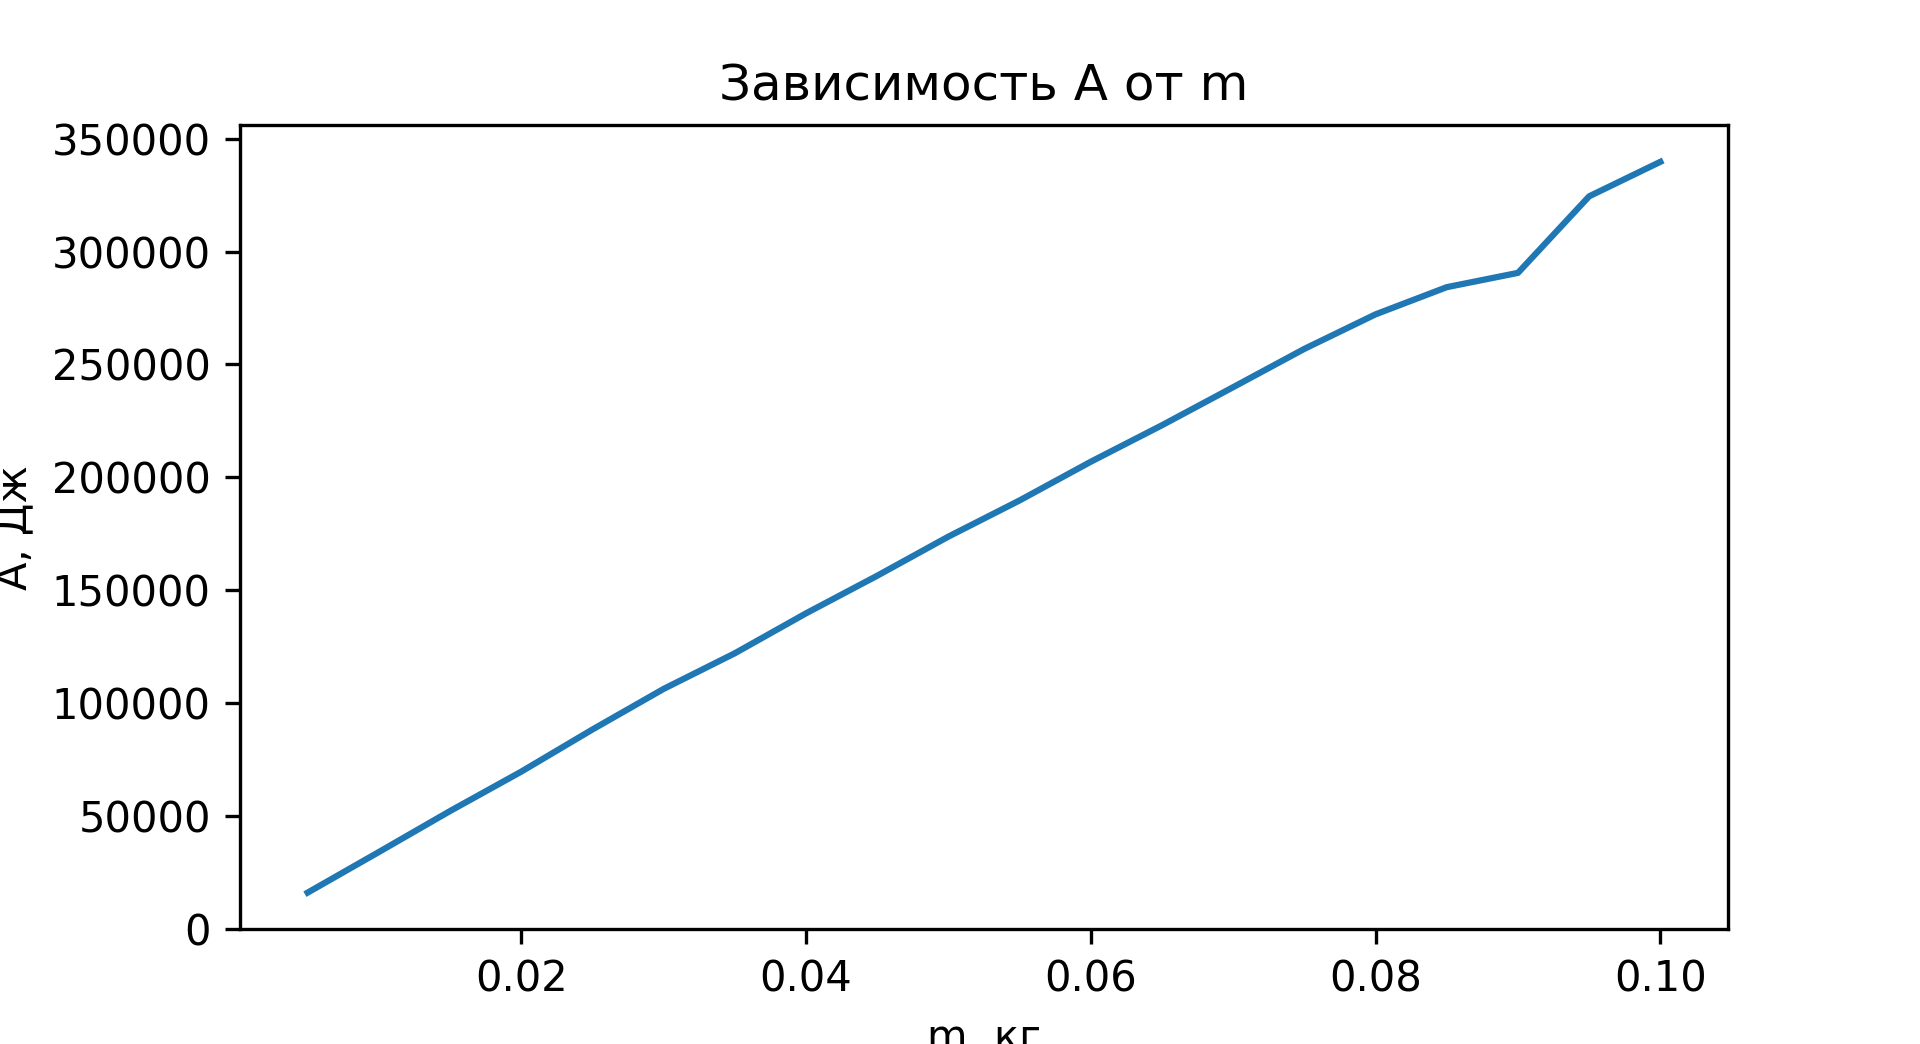
\includegraphics[width=0.8\textwidth]{fig_5}
    \end{center}

\end{figure}
На Рис. представлен график зависимости совершенной работы $A$ от массы испарившейся воды $m$.

График показывает практически линейную зависимость работы $A$ от массы $m$, что соответствует теоретическому ожиданию $A = Lm$.
\vspace{0.5cm}

% --- Section 8: Final Results ---
\section{Окончательные результаты}
\begin{enumerate}
    \item Экспериментальное значение удельной теплоты парообразования воды, найденное по наклону графика $A(m)$ (метод $\Delta A / \Delta m$):
        $L_{\text{эксп}} \approx \SI{2,14e6}{\text{Дж/кг}} = \SI{2,14}{\text{МДж/кг}}$.
    \item Табличное значение удельной теплоты парообразования воды:
        $L_{\text{табл}} = \SI{2,26}{\text{МДж/кг}}$.
    \item Относительное расхождение с табличным значением:
        \[ \delta L = \left| \frac{L_{\text{табл}} - L_{\text{эксп}}}{L_{\text{табл}}} \right| \times 100\% = \left| \frac{\SI{2,26}{\text{МДж/кг}} - \SI{2,14}{\text{МДж/кг}}}{\SI{2,26}{\text{МДж/кг}}} \right| \times 100\% \approx 5,2 \% \]
\end{enumerate}
\vspace{0.5cm}

% --- Section 9: Conclusion and Analysis ---
\section{Вывод и анализ результатов}
В ходе лабораторной работы были проведены измерения массы испарившейся воды и времени кипения для определения удельной теплоты парообразования воды.


На основе экспериментальных данных построена зависимость работы $A$, затраченной на испарение, от массы испарившейся воды $m$. График демонстрирует линейную зависимость, что подтверждает теоретическую формулу $A=Lm$.

Экспериментальное значение удельной теплоты парообразования, определенное как $L_{\text{эксп}} = \Delta A / \Delta m$, составило $L_{\text{эксп}} \approx \SI{2,12}{\text{МДж/кг}}$.

Сравнение полученного значения с табличным ($L_{\text{табл}} = \SI{2,26}{\text{МДж/кг}}$) показывает, что теория сходится с практикой.

Погрешность может быть вызвана рядом факторов:
\begin{itemize}
    \item Неточность в определении мощности теплопотерь $N_{\text{окр}}$ (зависит от точности измерения $M, \Delta t, \tau$ и постоянства условий охлаждения).
    \item Погрешности измерения массы $m$ и времени $t$.
\end{itemize}

\end{document}
